% !TEX root = ../MasterThesis_Onoe.tex
% 上記はただのコメントではなく親ファイルの場所を教えているので
% 消してしまうとファイルごとのタイプセットができなくなるので注意。
% 親ファイル名を変更したときはここも変更する。

\chapter{ビームテストによる評価試験} \label{sec:Beamtest}
本章では、CERN SPS加速器で行ったビームテストについて述べる。初めに3.1節でビームテストの概要について述べる。続いて3.2節でビームセットアップについて述べ、3.3節で実験結果についてまとめる。
\section{概要}
これまでに作成されたSiW-ECALの技術プロトタイプ(FEVおよびCOB)の性能評価実験を、2023年6月7日から2023年6月22日の期間にCERN SPS加速器のビームラインにて行った。本実験の主な目的は、電磁カロリメータとハドロンカロリメータの技術プロトタイプを同じビーム軸上に設置し、同時に運転を行いデータを取得すること、またこれまでの評価実験の中でも最高エネルギーのハドロンビームを用いて15層のSiW-ECALの評価を行うことの2点であった。また本実験におけるハドロンカロリメータは、同じくCALICEグループにおいてドイツやチェコが中心となって開発を進めているAHCALを用いた。以下では実験の詳細と、結果について述べる。
\subsection{ビームライン}
ビームテストは、フランスとスイスの国境付近に位置するCERN (図\ref{cernmapping})のSPS 加速器のビームラインを用いて行った。SPSは、現在 LHC の前段加速器として利用されており、陽子シンクロトロンから来た$\SI{26}{GeV}$の陽子を、周長7kmの加速器によって$400\sim \SI{450}{GeV}$まで加速している。SPSのビームラインでは、陽子ビームを固定ターゲットに入射することで、電子、ミューオン/パイ中間子の2次ビームを運動量$10\sim \SI{400}{GeV}$で得ることができる。本実験ではこれらのビームを用いて、NorthエリアにあるH2Aビームラインで実験を行った。実験に用いたビームパラメータを表 3.1に示す。\\
\begin{figure}[H]
	\begin{center}
 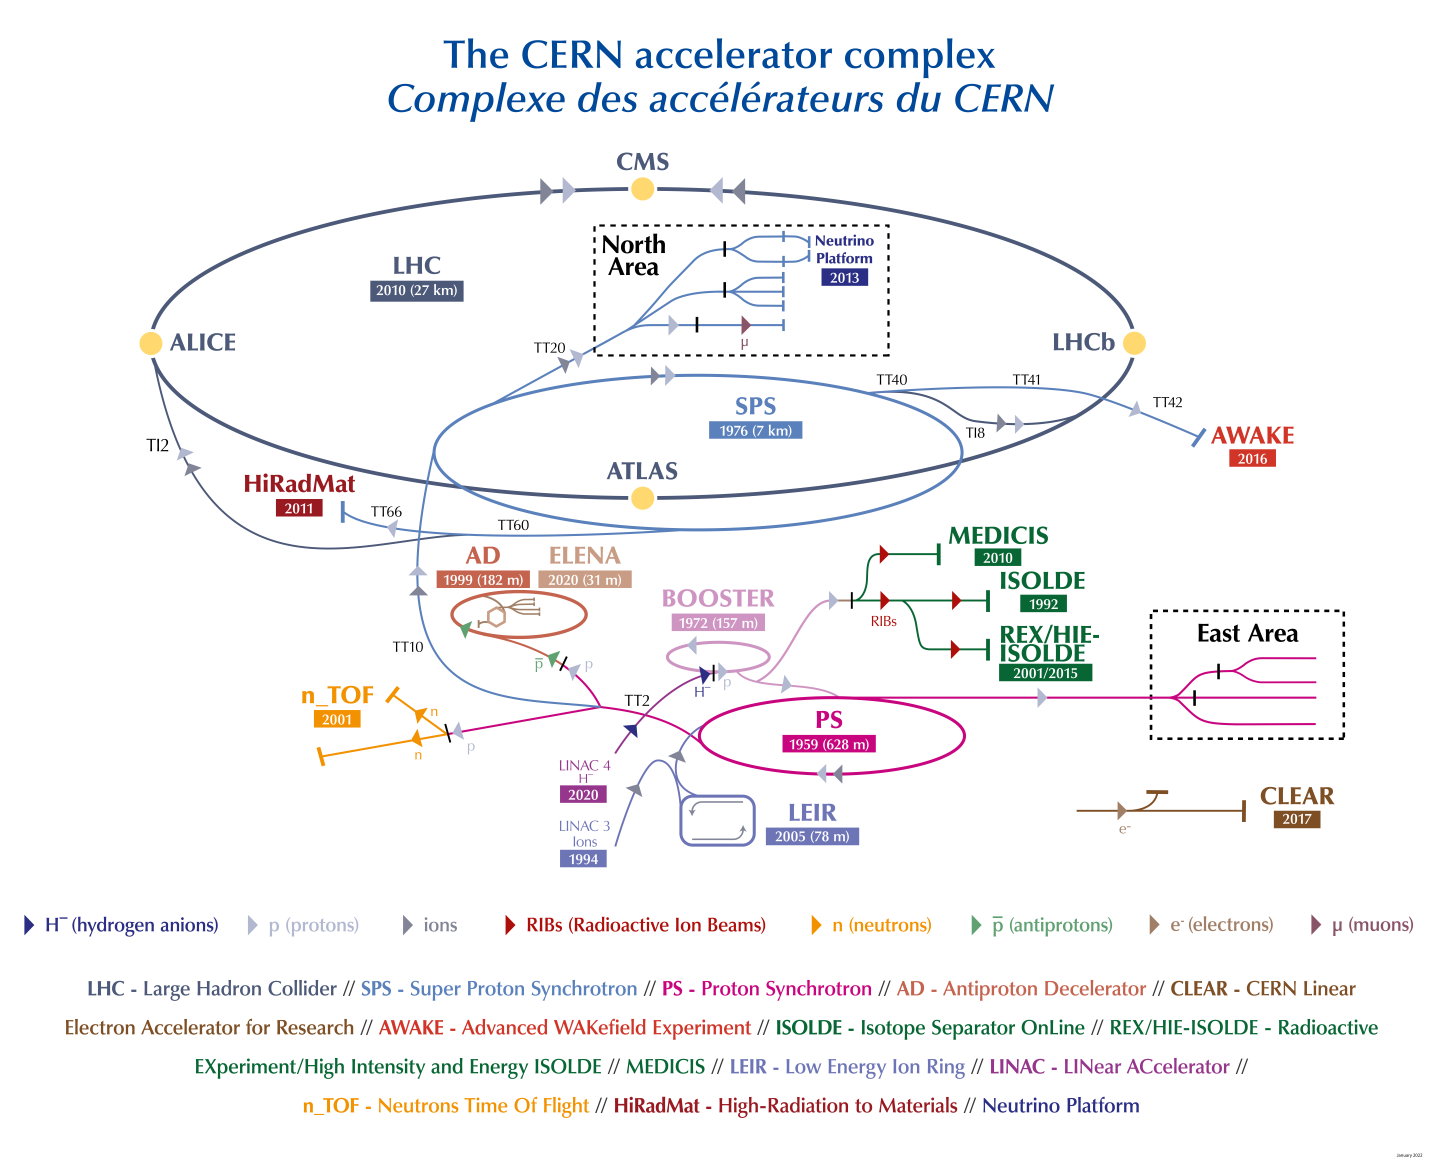
\includegraphics[keepaspectratio, scale=0.7]
 	{Figure/Beamtest/cern.png}
 		\caption{CERN加速器の全体図~\cite{cernmap}}
		\label{cernmapping}
	\end{center}
\end{figure}
\begin{table}[H]
 \centering
 \begin{tabular}{c c}
 \hline
運動量 & 10-200$[ \mathrm{GeV}/ c ]$\\
電子のpurity & 10-99.5\%\\
Max $\delta p / p$  & $2\%$\\
ビームの高さ & 2460$[ \mathrm{mm}]$\\
 \hline
 \end{tabular}
 \caption{H2Aビームラインにおけるビームパラメータ}
\end{table}

\section{実験セットアップ}
\subsection{測定機器のセットアップ}
本実験でのセットアップの概観を図\ref{setup1}に示す。図中右手からビームが照射され、ILDの構成と同様に上流側にSiW-ECALが、下流側にAHCALを設置した。SiW-ECALのプロトタイプは、FEVが13層(うちFEV10が1層、FEV11が3層、FEV12が2層、FEV13が7層)COBが2層を組み合わせた計15層からなる検出層と鉛板15層の吸収層からなるモジュールを組み立てた。今回のビームテストの検出層は、最も良い性能が期待できるFEV13を前方に設置し、性能比較のためにCOBを加えた構成となった。15層の検出層において、センサーと読み出しボードに供給する電源は、15層に対して図\ref{setup2}左のように並列で印加した。また、信号はカプトンケーブルを通して15層分の信号を一括してCOREモジュールに送り、PCで読み出しを行った。また、AHCALもサンプリング型ハドロンカロリメータであり、鉄の吸収層とシンチレータ検出層によって構成されていて、読み出しはシンチレータに統合されたエレクトロニクスによって行われる。
\begin{figure}[H]
\begin{center}
 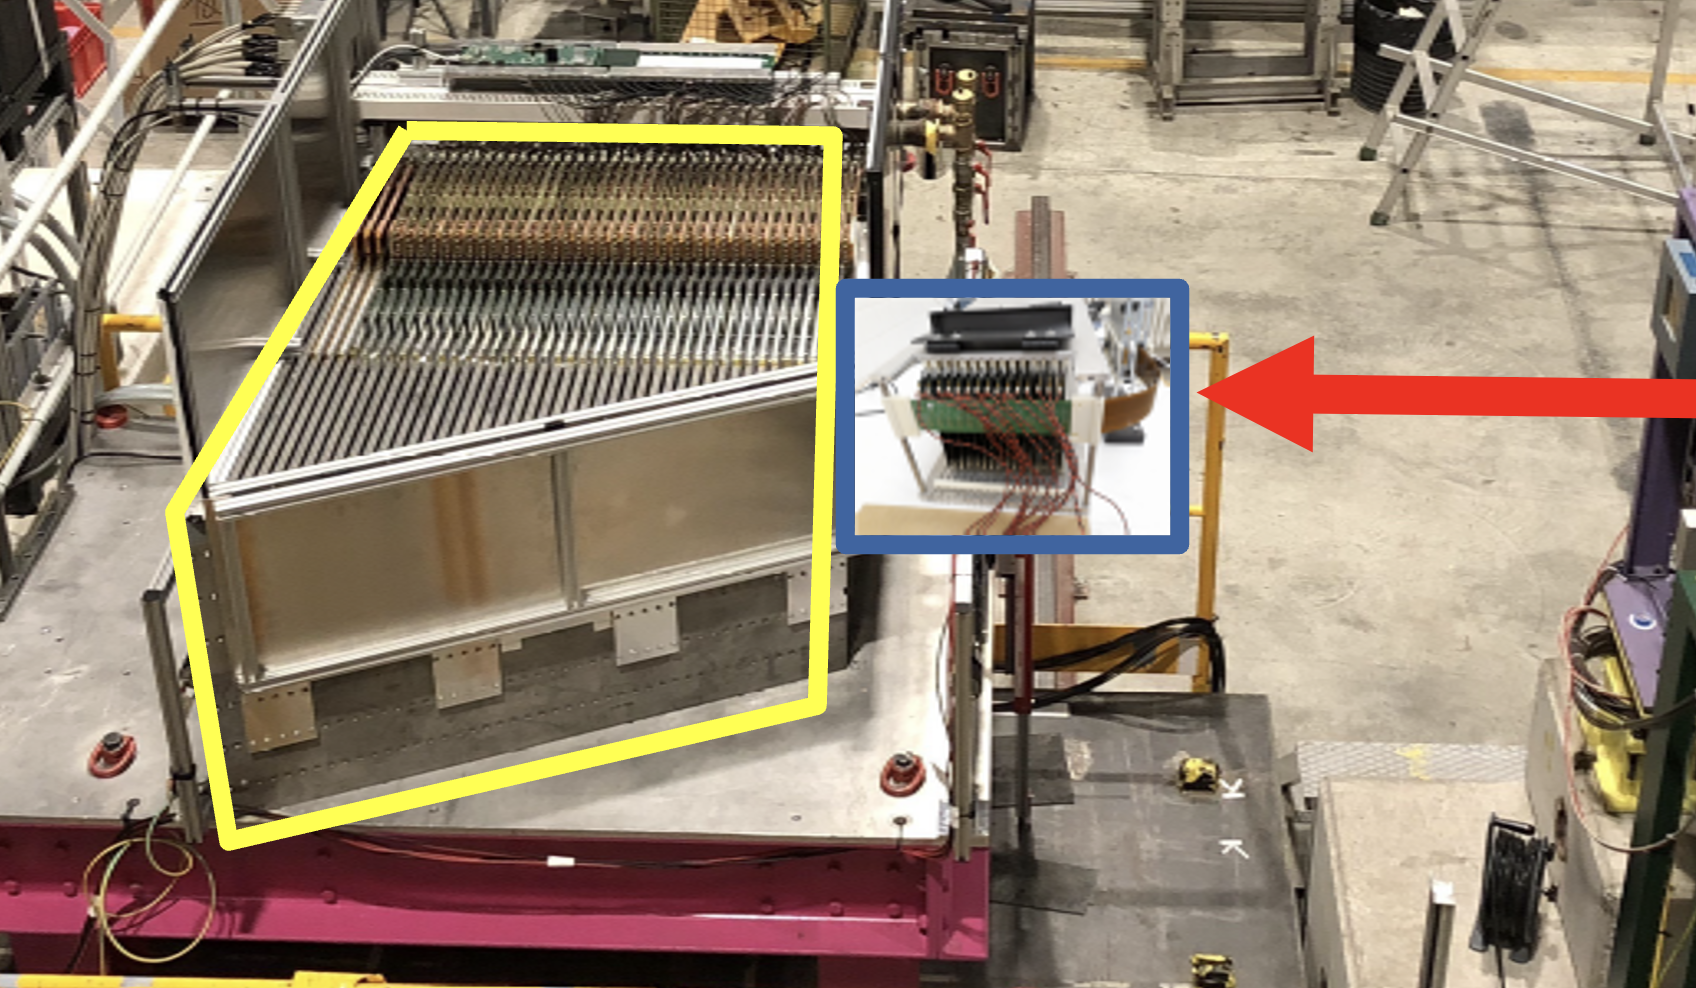
\includegraphics[keepaspectratio, scale=0.3]
 	{Figure/Beamtest/setup1.png}
 		\caption[セットアップの全体図]{セットアップの全体図。黄枠:AHCAL、青枠:SiW-ECAL、赤:ビーム位置}
		\label{setup1}
		\end{center}
\end{figure}

\begin{figure}[H]
\begin{center}
 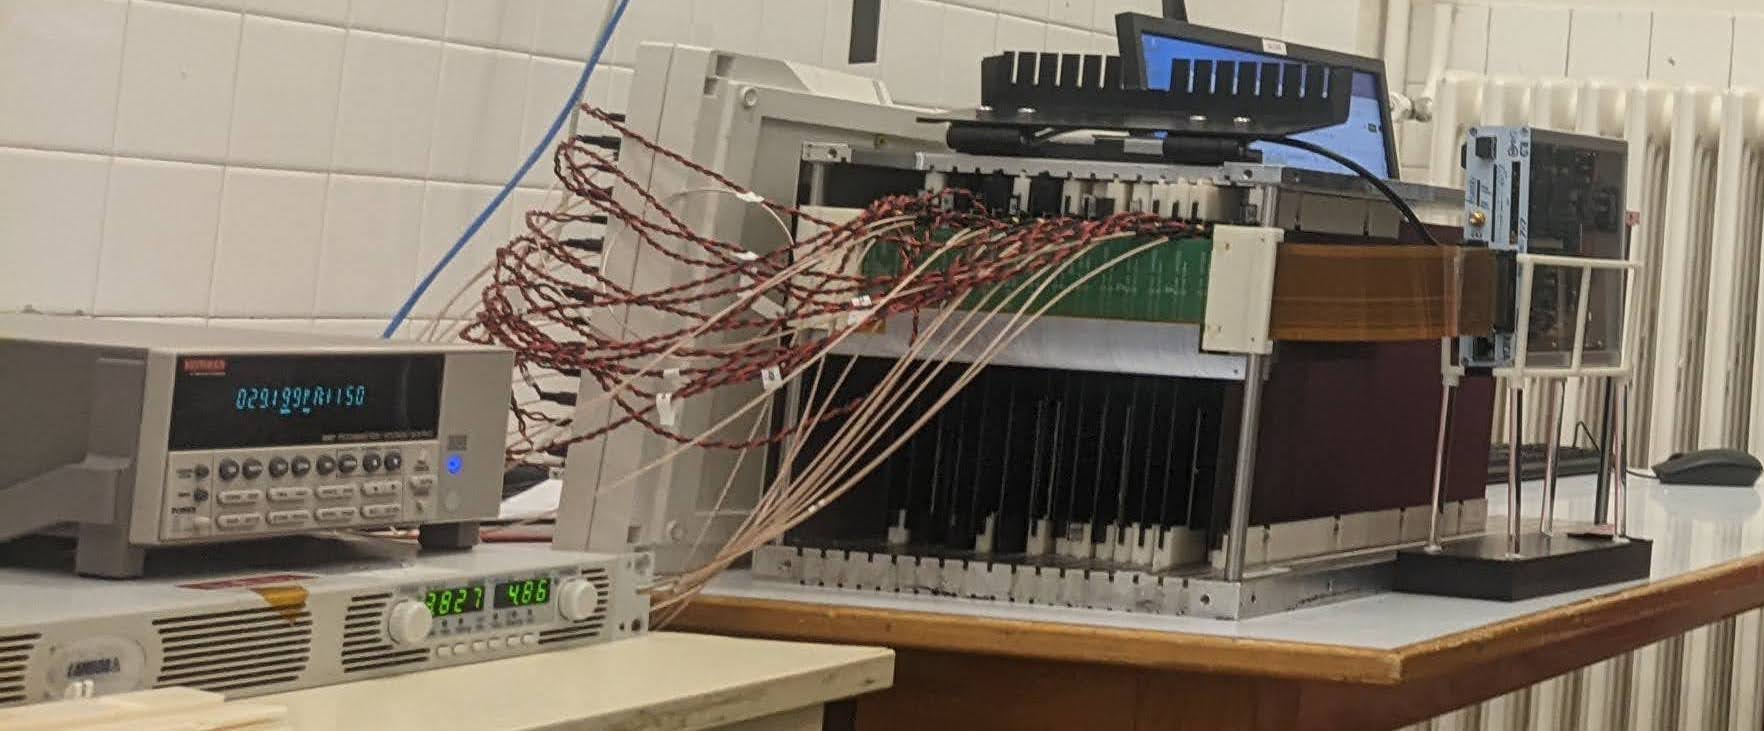
\includegraphics[keepaspectratio, scale=0.2]
 	{Figure/Beamtest/setup2.png}
 		\caption{SiW-ECALのプロトタイプモジュールと電源供給、読み出しシステム}
		\label{setup2}
\end{center}
\end{figure}

\begin{table}[H]
 \centering
 \begin{tabular}{|c|c|c|c|}
 \hline
層数 & ボードの種類 & ウェハー厚み$[\mu m]$ & タングステン厚み[mm]\\
 \hline
 \hline
0 & FEV13 & 650 & 4.2\\
1 & FEV13 & 650 & 4.2\\
2 & FEV13 & 650 & 4.2\\
3 & FEV13 & 650 & 4.2\\
4 & FEV13 & 500 & 4.2\\
5 & FEV13 & 500 & 4.2\\
6 & COB & 500 & 4.2\\
7 & FEV12 & 500 & 4.2\\
8 & COB & 500 & 5.6\\
9 & FEV12 & 500 & 5.6\\
10 & FEV11 & 320 & 5.6\\
11 & FEV11 & 320 & 5.6\\
12 & FEV10 & 320 & 5.6\\
13 & FEV13 & 320 & 5.6\\
14 & FEV11 & 320 & 5.6\\
 \hline
 \end{tabular}
 \label{layer}
 \caption{SiW-ECALのレイヤー構成 (0層目がビーム上流側) }
\end{table}
\subsection{信号読み出し}
SiWECALとAHCALは独立にDAQを行うが、本実験ではEUDAQという読み出しフレームワークによってAHCALと同期した読み出しを行った。EUDAQでは、SiWECALとAHCALの間でClock and Control Card (CCC) を同期させており、CCCではクロック、スタート、ストップ信号をPCへ送っているため、PC上で時間情報である Bunch Crossing ID (BCID) が同じイベントを収集することができる。\\
また、SiWECALでは専用のDAQソフトウェア~\cite{ecalsoft}が稼働しており、DAQのみでなくチャンネル単位での閾値の設定やイベントのモニター (図\ref{monitor}) が可能となっている。データはraw形式で保存され、解析用のソフトウェアを通してツリー形式にデータを保存したrootファイルへ変換し解析に利用することができる。
\begin{figure}[H]
\begin{center}
 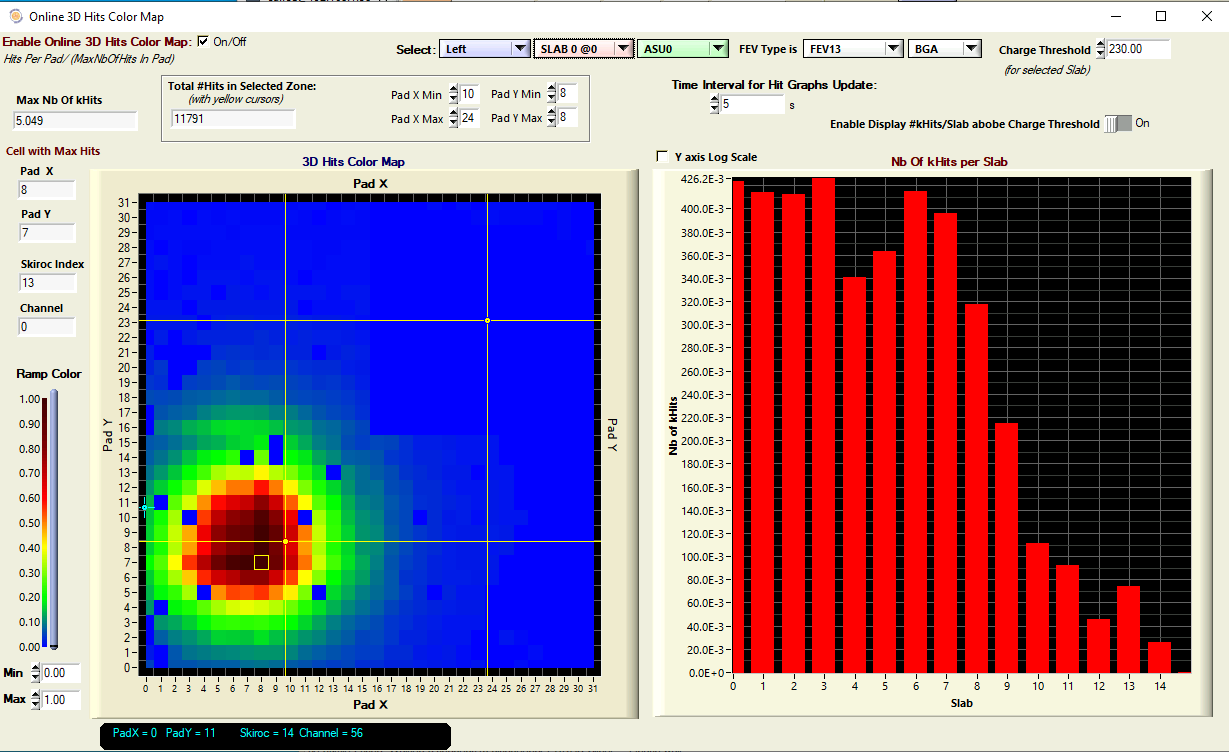
\includegraphics[keepaspectratio, scale=0.2]
 	{Figure/Beamtest/monitor.png}
 		\caption[SiW-ECALのイベントモニター]{SiW-ECAL読み出しソフトウェアにおけるイベントモニター (左) ヒットマップ (右) 各層あたりのヒット数}
		\label{monitor}
\end{center}
\end{figure}
\section{実験結果}
\subsection{検出器応答}
各runに対して層ごとのヒットマップを作成し、各層の応答を確認した。作成したヒットマップを図\ref{hitmap}に、runの詳細を表3.3に示す。ビームはヒットマップ左下のセンサーを中心に照射を行った。\\
電子ビームは相互作用を起こし電磁シャワーを形成するため、ヒット領域が大きくなっていることが確認できる。またミューオンビームは、基本的に単体では電磁シャワーを形成しないものの、ヒットマップではビームサイズが大きくなっている。これは、ビームライン中においてパイオンの崩壊などによってビーム内の位置分布が広がることによる影響であると考えられる。また白く抜けている箇所はノイズが多いためマスクしている、あるいは信号がないチャンネルであるが、ビームの種類によらず全体を通して4つほど四角く抜けている部分が確認できる。これは1枚のセンサーの場所と対応しており、導電性接着剤の剥離、高電圧の接続不良、センサーの損傷などによるものである。\\
さらにビームのエネルギーを上げていくと、$\SI{80}{GeV}$以上のエネルギーで図\ref{hitmap} (b)第6層のような、1センサー全体にヒットが集中してしまう現象が確認された。エネルギーが大きくなった場合にはセンサーに入ってくる信号が多くなることから、センサー周辺での放電等が原因として考えられるが、現在調査を行なっている。
\begin{figure}[H]
  \begin{minipage}[b]{0.45\linewidth}
    \centering
    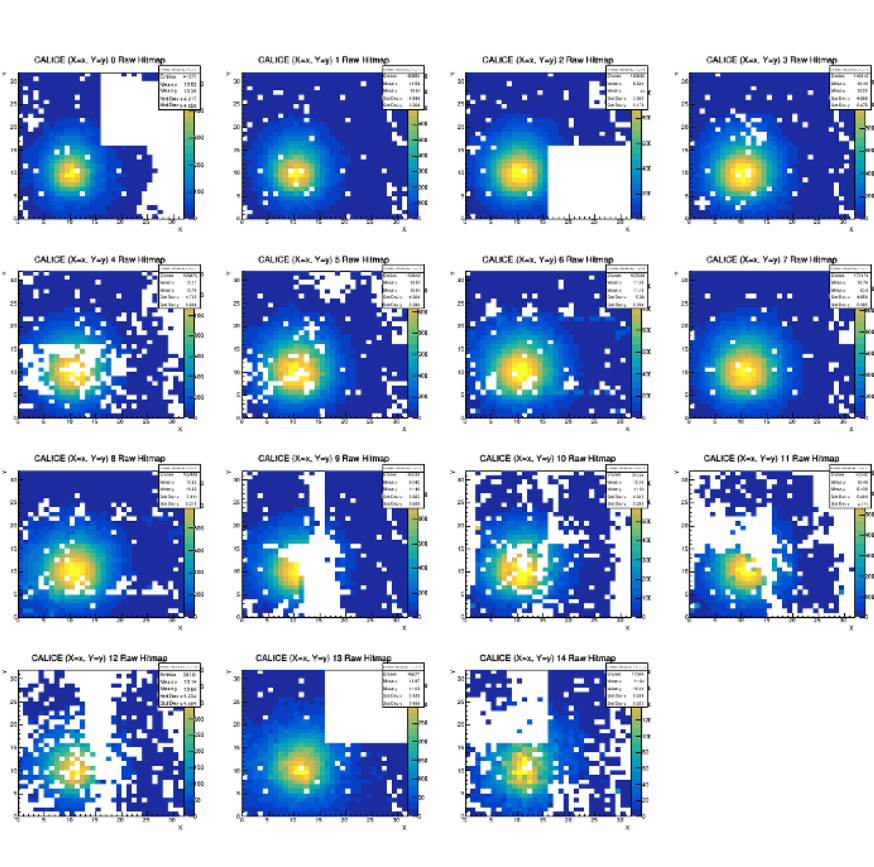
\includegraphics[keepaspectratio, scale=0.2]{Figure/Beamtest/hitmap_e20.png}
    \subcaption{$\SI{10}{GeV}$電子ビーム}
  \end{minipage}
    \begin{minipage}[b]{0.45\linewidth}
    \centering
    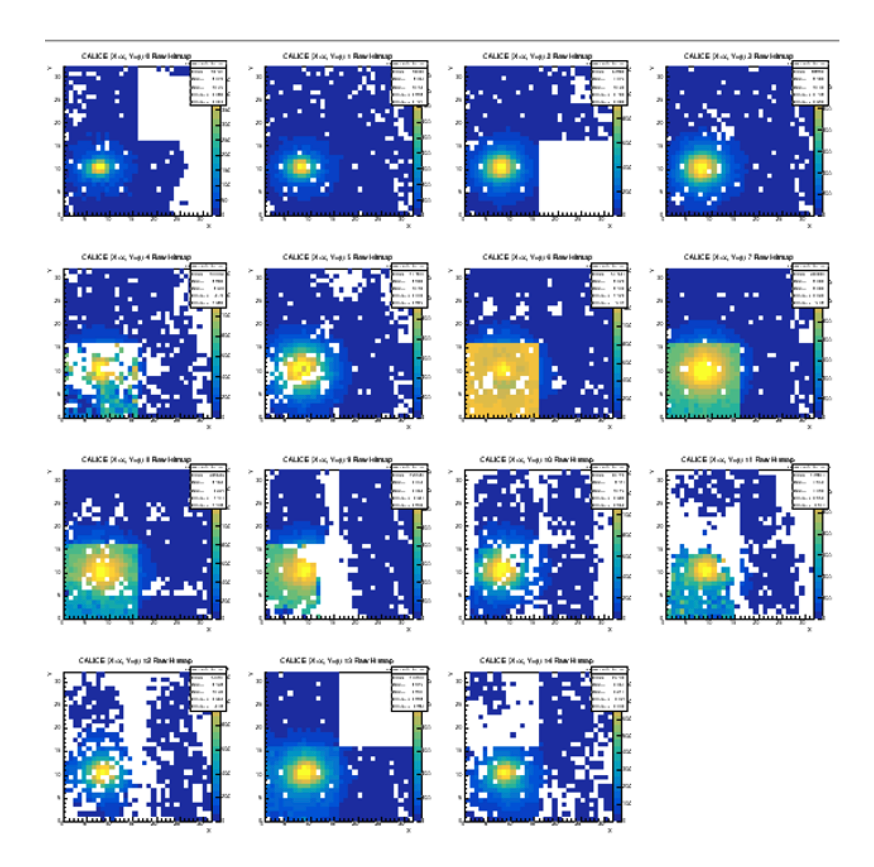
\includegraphics[keepaspectratio, scale=0.2]{Figure/Beamtest/hitmap_e150.png}
    \subcaption{$\SI{150}{GeV}$電子ビーム}
  \end{minipage}
  \begin{minipage}[b]{0.45\linewidth}
    \centering
    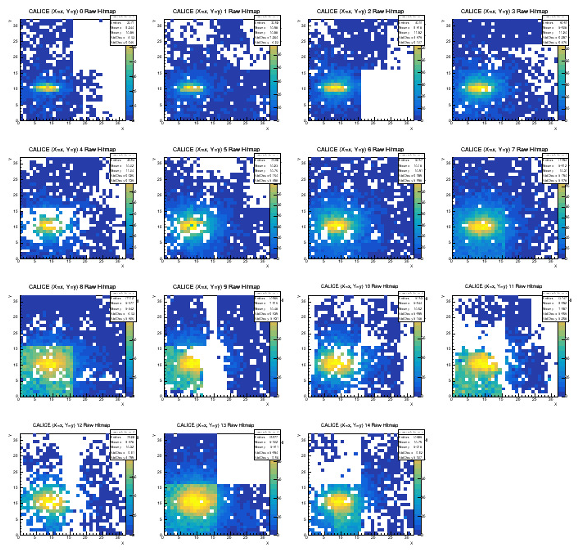
\includegraphics[keepaspectratio, scale=0.2]{Figure/Beamtest/hitmap_mu150.png}
    \subcaption{$\SI{150}{GeV}$ミューオンビーム}
   \end{minipage}
   \hfill
  \begin{minipage}[b]{0.45\linewidth}
    \centering
    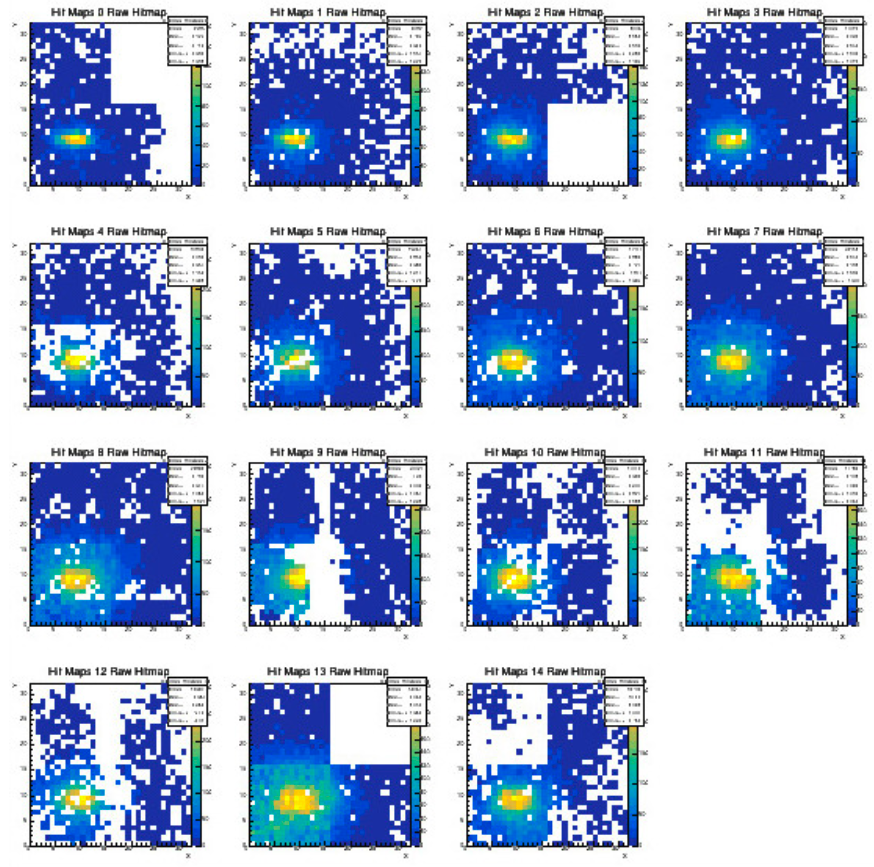
\includegraphics[keepaspectratio, scale=0.2]{Figure/Beamtest/hitmap_pi150.png}
    \subcaption{$\SI{150}{GeV}$パイ中間子ビーム}
  \end{minipage}
  \caption[各ビーム種類におけるヒットマップ]{各ビーム種類におけるヒットマップ。左上から0層右上が3層、右下が14層と順に並んでいる。}
  \label{hitmap}
\end{figure}

\begin{table}[H]
\centering
\begin{tabular}{ c c c c c c}
\hline
図番号 & ビーム種類 & エネルギー$ [\mathrm{GeV}] $ & トリガー数 & データ取得時間 [分] & run番号 \\
\hline \hline
(a) & 電子 & 10 & 23790 & 30 & 90289 \\
(b) & 電子 & 150 & 40542 & 30 & 90344 \\
(c) & ミューオン & 150 & 179078 & 30 & 90484 \\
(d) & パイオン & 200 & 64208 & 30 & 90341 \\
\hline
\end{tabular}
\caption{ヒットマップの作成において使用したrunの詳細}
\end{table}

\subsection{ペデスタル・Retriggering}
続いて、ペデスタルの解析を行った。ペデスタルとは信号が全くきていない時(トリガーが入っていない時)の信号の大きさで、エレクトロニクス由来のノイズ等によってその値の幅は変化する。信号のゲインなどは、ペデスタルからどれだけ離れているかで定義するため、 それぞれのチャンネルでペデスタルがどのようになっているか調べることは重要な情報となる。一般的にぺデスタルは図\ref{ped}のようにガウス関数でフィッティングすることができ、その中央値はペデスタル信号の大きさを、標準偏差はその揺らぎの大きさ (ノイズ) に相当する。図\ref{pedestal}に各エネルギーの電子ビームのrunにおける同じチャンネルのペデスタルを示した。この図より、ビームのエネルギーに依らずぺデスタルの中央値は一定の値を取ることが確認された。また、runの長さは同じであるものの、エネルギーが大きいビームでは、ペデスタルの信号数が多くなった。さらにペデスタルの波形に注目すると、低エネルギーになるにつれてピークが2つに分かれてきていることも確認できる。これはこの節の後半に示すダブルぺデスタルであると考えられる。\\
\begin{figure}[H]
\begin{center}
 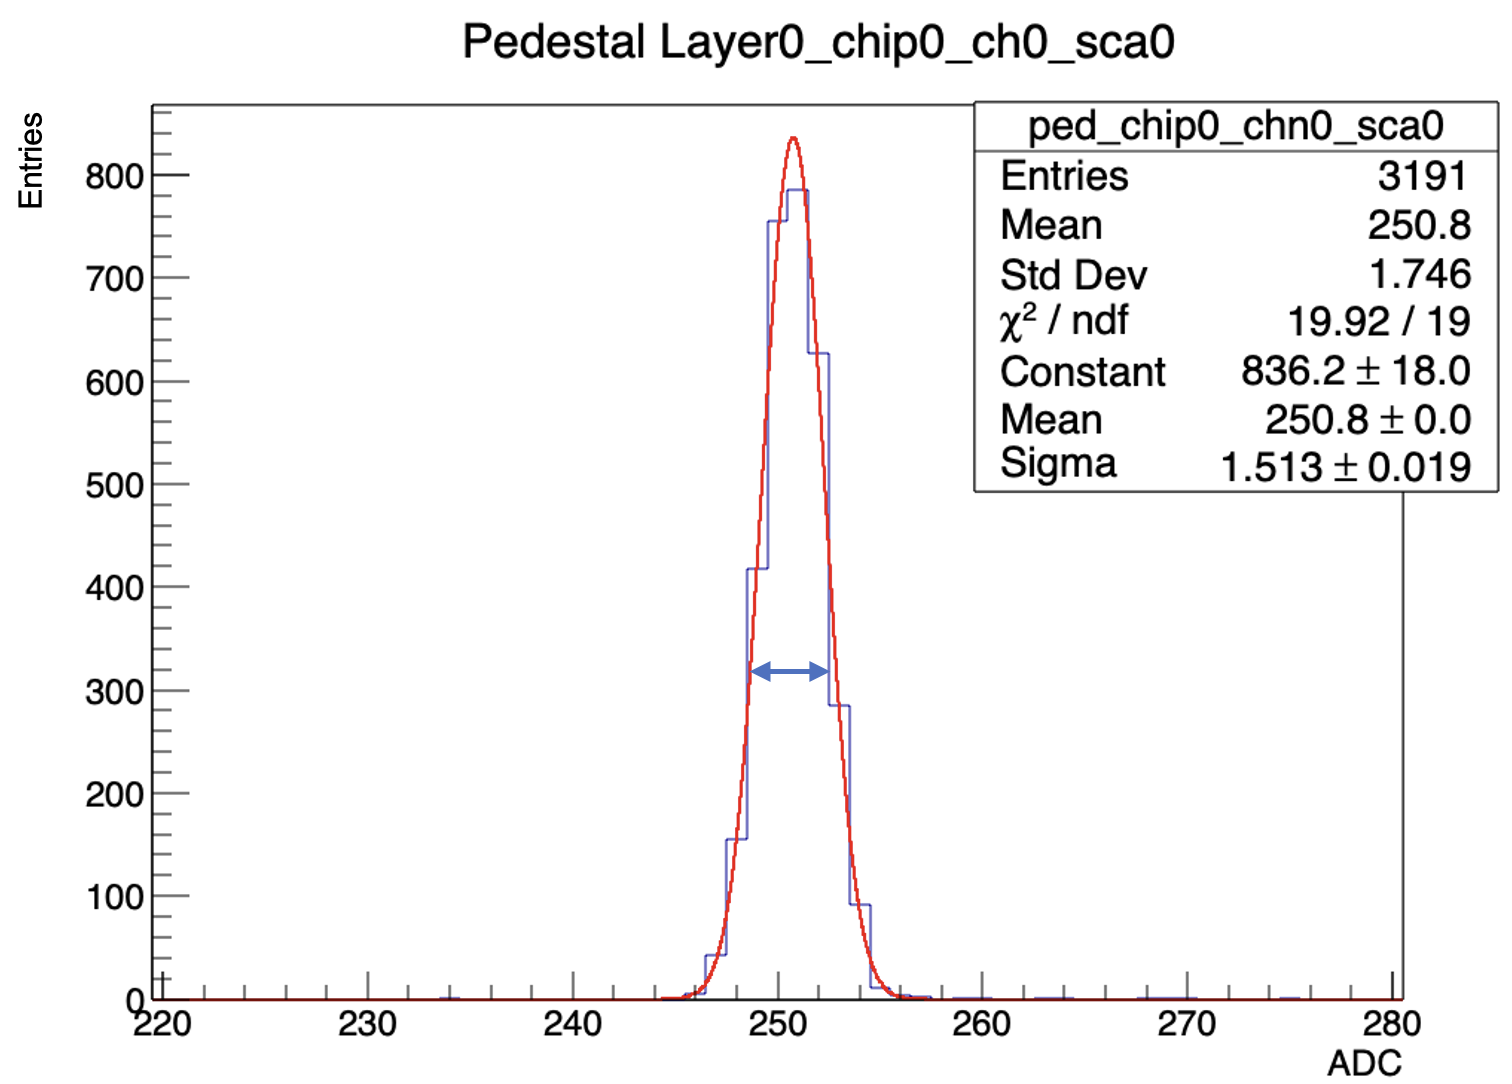
\includegraphics[keepaspectratio, scale=0.3]
 	{Figure/Beamtest/ped.png}
 		\caption{ペデスタルヒストグラムの例}
		\label{ped}
\end{center}
\end{figure}
\begin{figure}[H]
\begin{center}
 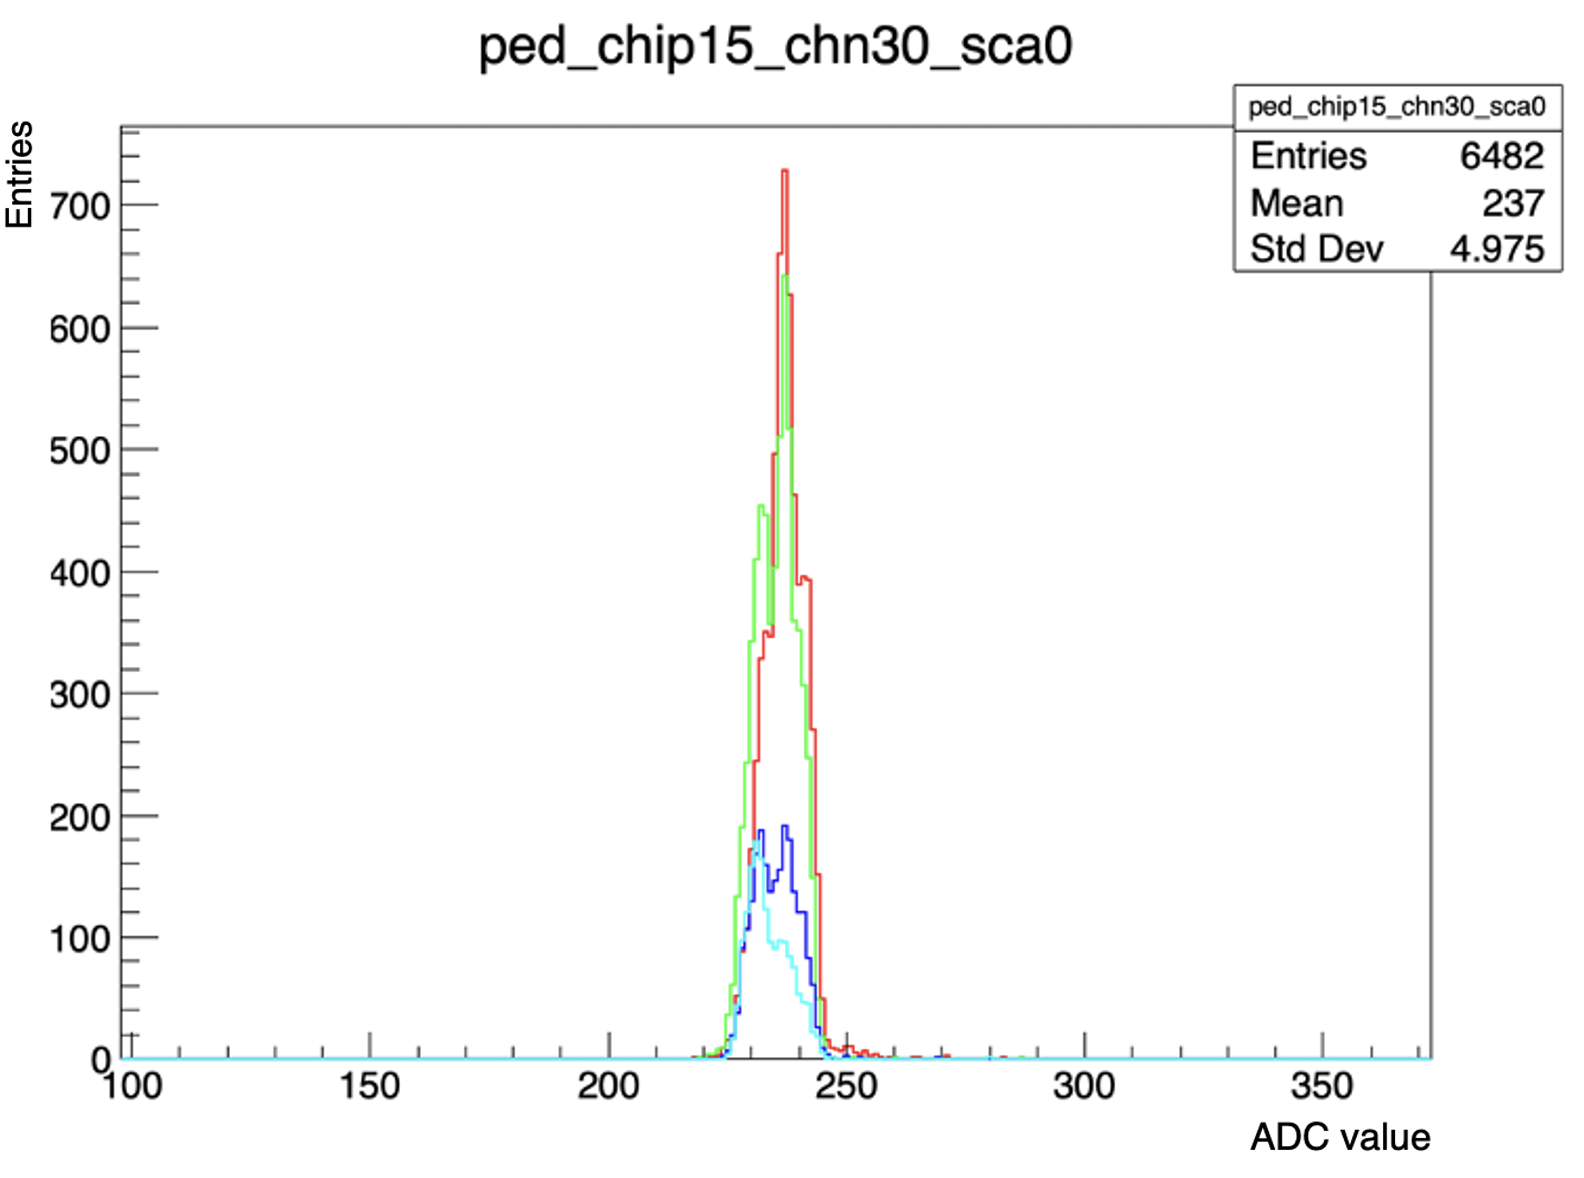
\includegraphics[keepaspectratio, scale=0.3]
 	{Figure/Beamtest/pedestal.png}
 		\caption[異なるビームエネルギーにおけるペデスタル]{$水色: \SI{40}{GeV}/紺: \SI{60}{GeV}/緑: \SI{100}{GeV}/赤: \SI{150}{GeV}$の電子ビームにおけるペデスタル}
		\label{pedestal}
\end{center}
\end{figure}
また、各チャンネルにおけるペデスタルの中央値の大きさと標準偏差を図\ref{means}に示す。図は横軸がチップのインデックスに対応し、縦軸がチャンネルのインデックスに対応している。また、黒枠は一つの層を表している。この図より、ペデスタルの中央値が層、チャンネルによって異なることが確認された。そのためぺデスタルの分布を確認したところ、チャンネルによって図\ref{dp}に示すような2つのピークを持つペデスタルが確認された。このペデスタルピークが2つ見える現象をダブルぺデスタルと呼んで調査・解析を行なった。また、今回の実験によって取得されたデータには、トリガーが入っているもののヒットのイベントが記録されていないデータがあり、この現象をRetriggeringと呼んでいる。Retriggeringが発生してしまうと、memory cellが偽物のヒットで満たされてしまうため、本来のデータが収集できないという問題が発生してしまい、DAQにおいて非常に重要な課題となっている。そのためダブルぺデスタルの状況とRetriggeringの発生について詳細に解析を行った。\\

\begin{figure}[H]
\begin{center}
 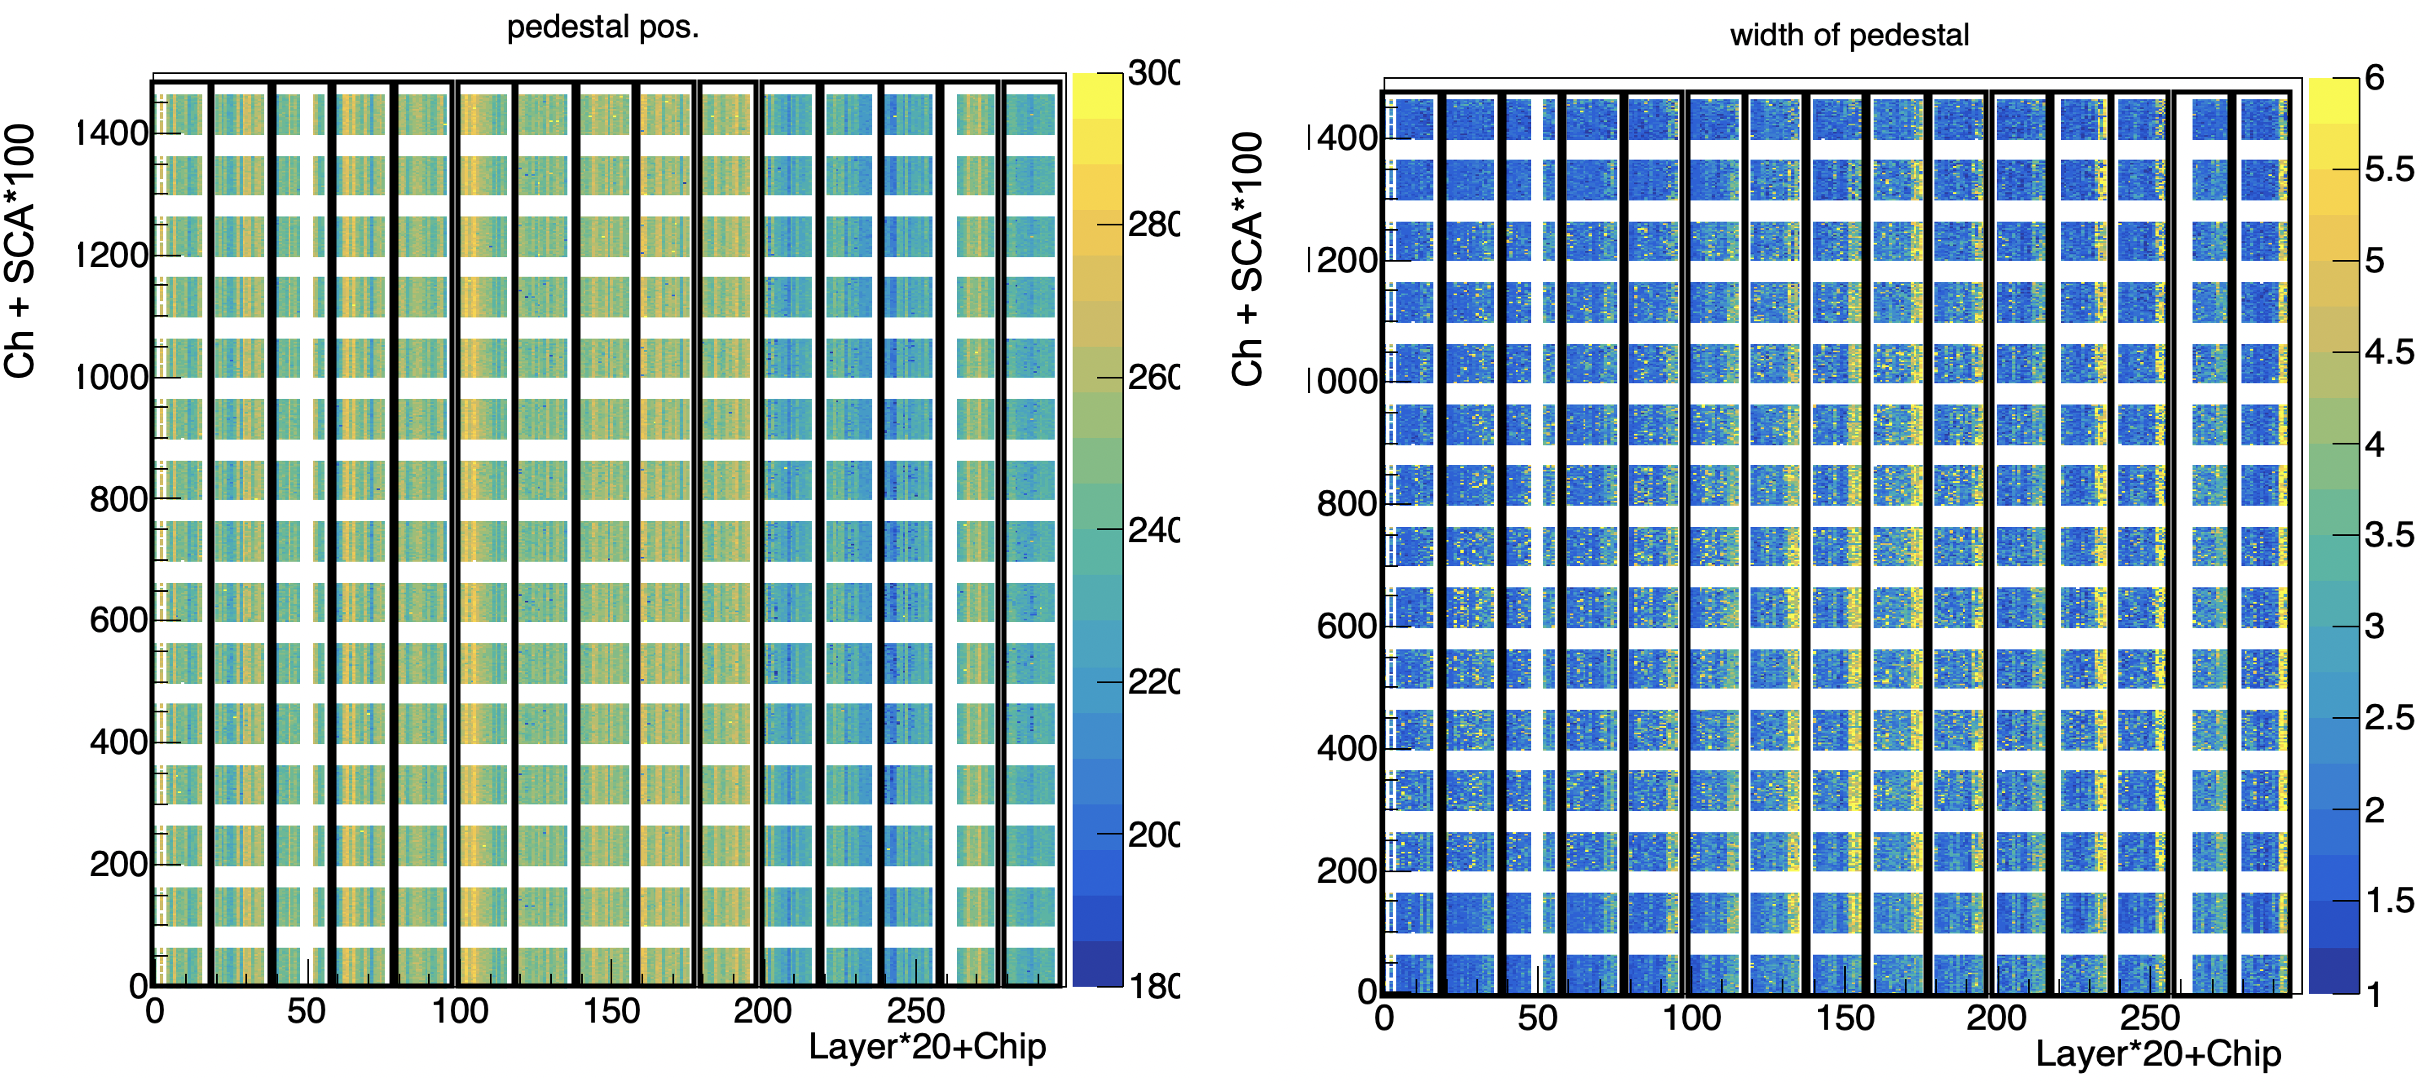
\includegraphics[keepaspectratio, scale=0.3]
 	{Figure/Beamtest/ped_pos.png}
 		\caption[全チャンネルに対するペデスタルのフィッティング]{ペデスタルをガウス関数フィットした際のパラメータ。横軸がチップを、縦軸がチャンネル番号を表しており、それぞれ全層、全SCAでの可視化のため、層数やSCAをかけた値となっている。(左) ガウス関数の中央値 (右) ガウス関数の幅の大きさ}
		\label{means}
\end{center}
\end{figure}
\begin{figure}[H]
\begin{center}
 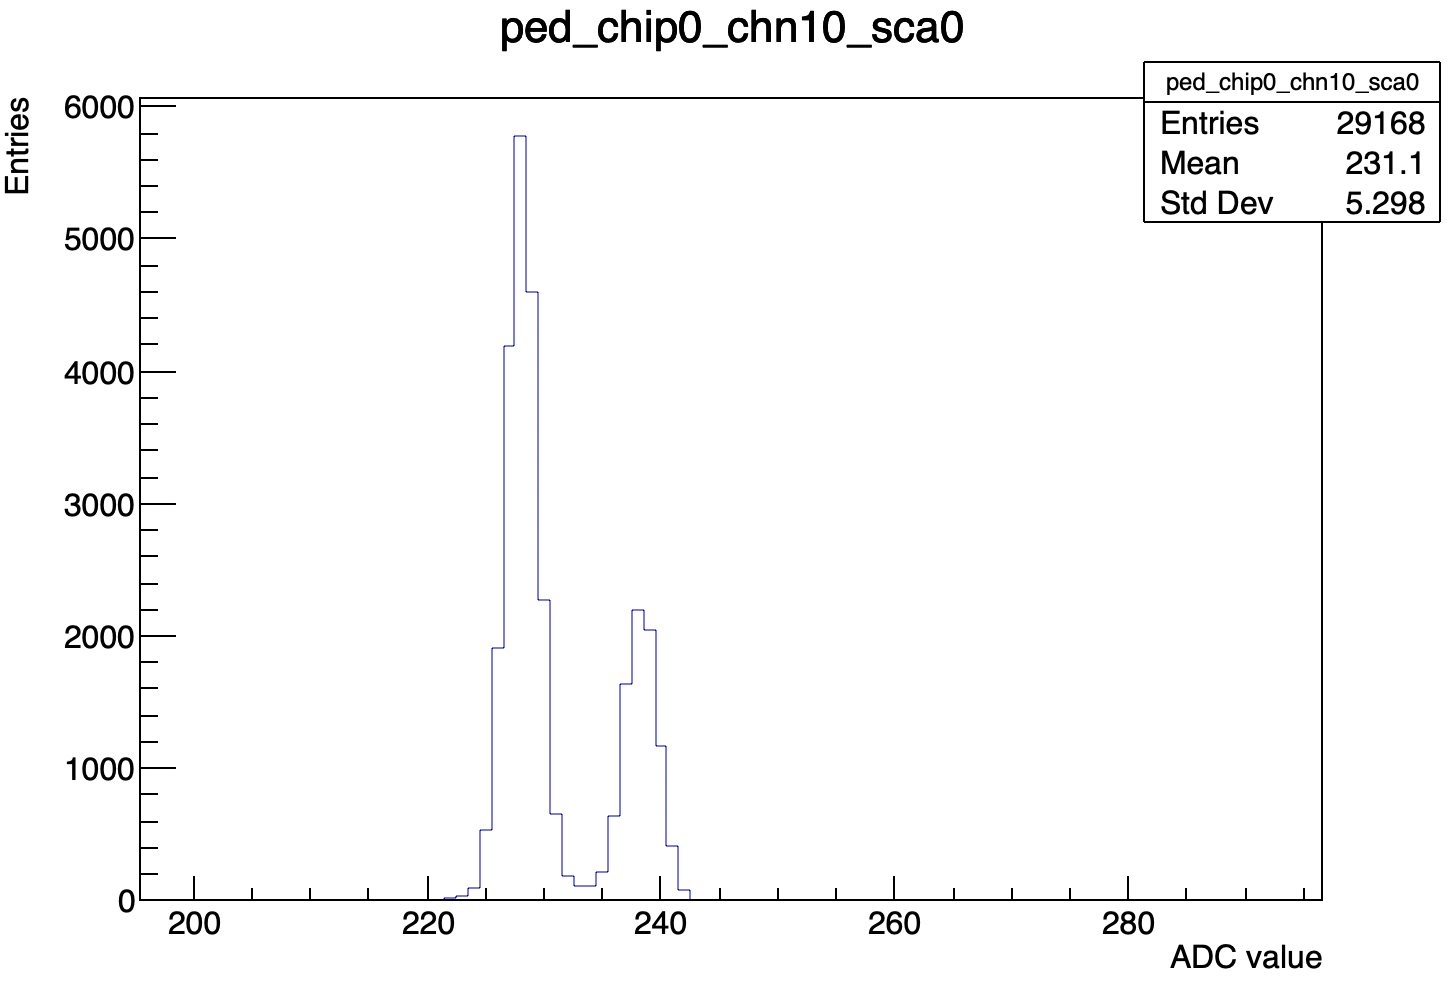
\includegraphics[keepaspectratio, scale=0.3]
 	{Figure/Beamtest/dp.png}
 		\caption{ダブルペデスタルの例}
		\label{dp}
\end{center}
\end{figure}
ペデスタルはトリガーが入っていない時の信号であるため、解析にはトリガーが少ないことが想定されるミューオン$\SI{150}{GeV}$のrunを用いた。はじめに各チャンネルにおけるADCの情報から、トリガーが入っていない条件に加えRetriggeringである可能性が高い連続したBCIDをカットする条件をかけることで、ペデスタルのヒストグラムを作成し、ピークの数を調査した。続いて、ピークが2つ以上見られるチャンネルに対して、各ピークに対してガウス関数でフィッティングを行い、中央値からペデスタルの信号の大きさを特定した。ピーク同士の信号の大きさはチャンネルによって異なり、図\ref{dpmap}に各チャンネルにおいてダブルペデスタルが発生した時の、2つのペデスタル信号の大きさの差を示す。1つのマップは1つの層に対応しており、左上から0層右上が3層、右下が14層と順に並んでいる。また、ダブルぺデスタルが発生したチャンネルには、2つのペデスタル信号の大きさの差をカラーバーに示している。このマップから、10、11、12、14層でダブルぺデスタルが多く発生していることが確認できる。これは10、11、12、14層がそれぞれ、FEV11、FEV11、FEV10、FEV11と以前のバージョンのFEVを使用しており、過去の配線のアップデートによってダブルぺデスタルの原因が大きく解消されていることが推測される。また、全層を通してダブルぺデスタルはボードの左下部分を中心に発生していることが確認できた。

\begin{figure}[H]
\begin{center}
 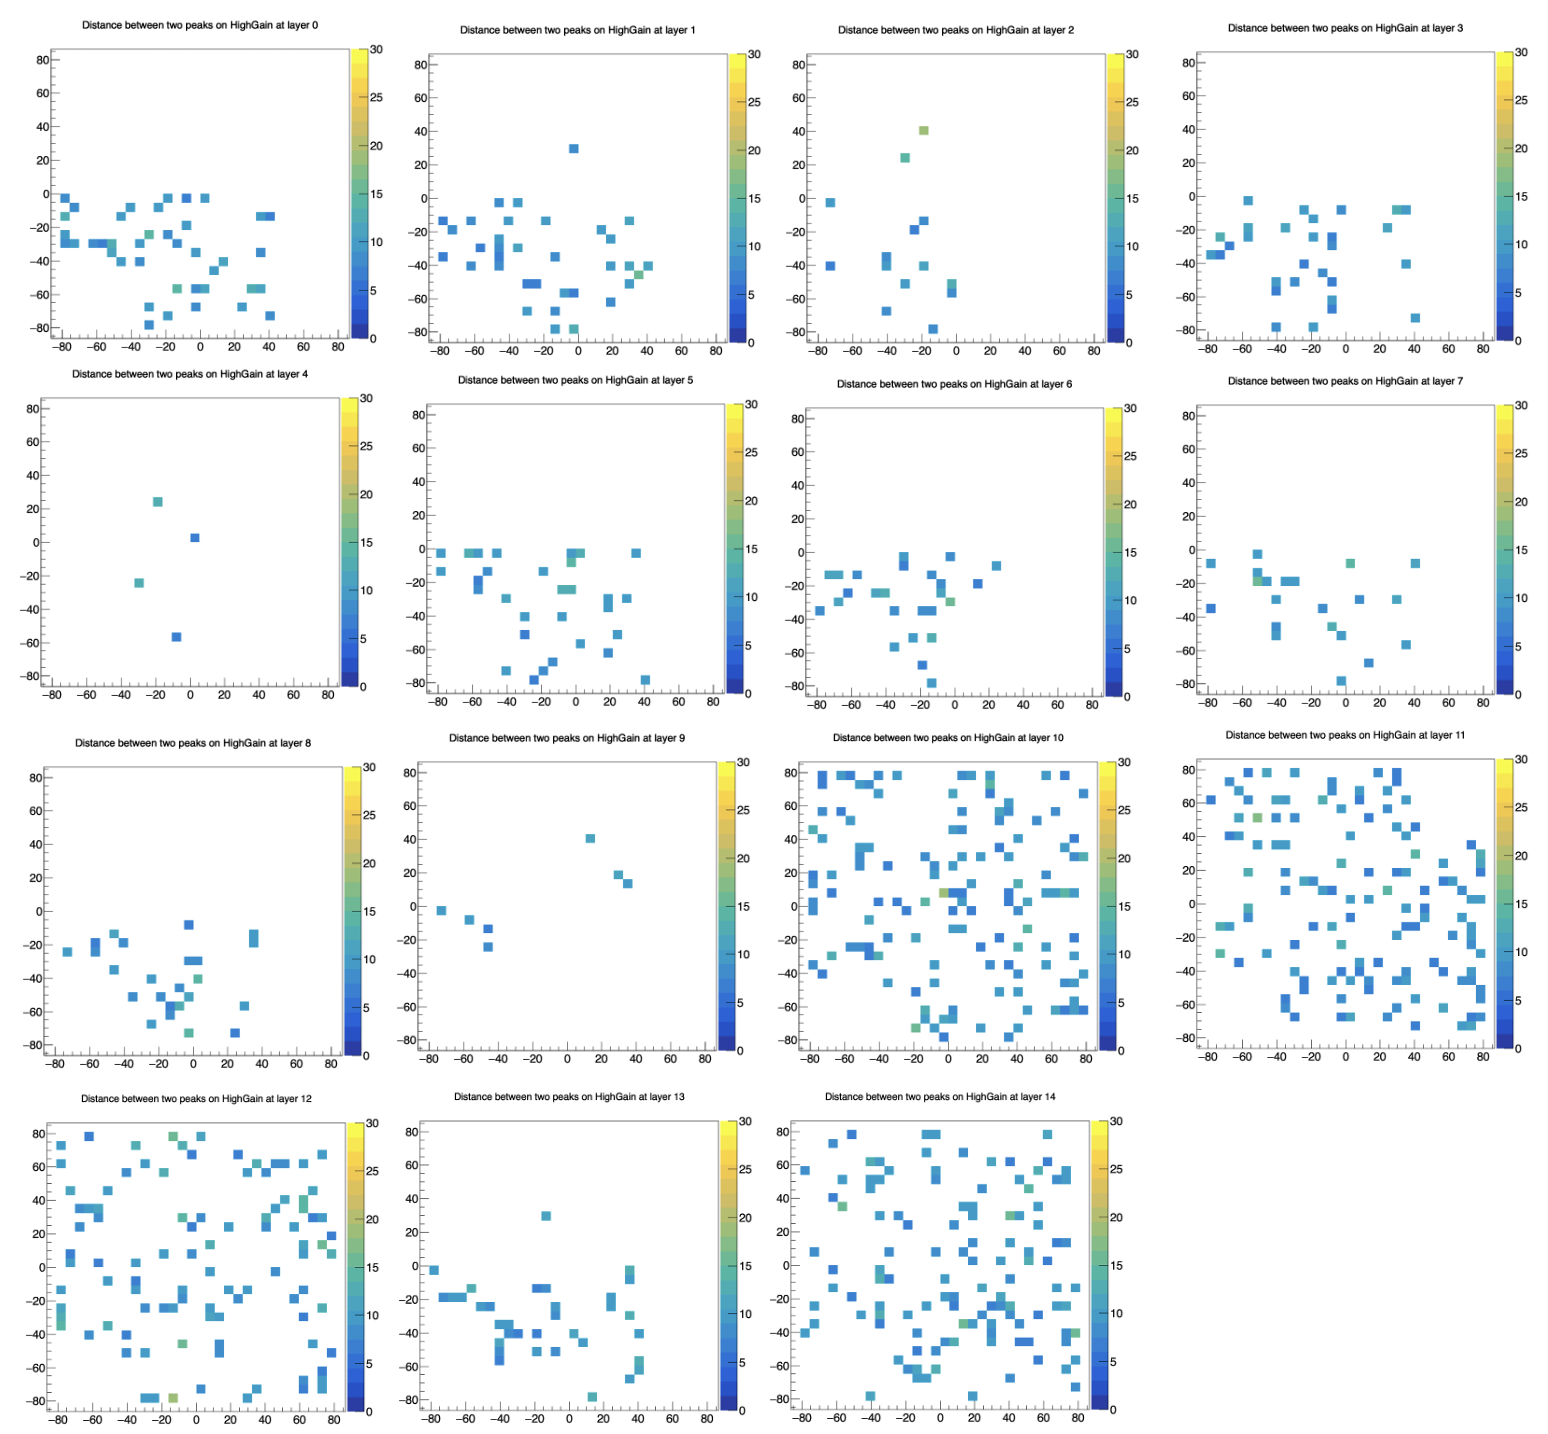
\includegraphics[keepaspectratio, scale=0.45]
 	{Figure/Beamtest/dpmap.png}
 		\caption[各層におけるダブルペデスタルのピーク間距離]{各層におけるダブルペデスタルのピーク間距離。左上から0層右上が3層、右下が14層と順に並んでおり、x,y軸の値はセンサー中心を原点とした、各チャンネルの座標を表す。}
		\label{dpmap}
\end{center}
\end{figure}

また、同一のデータを用いてTriggerとRetriggeringのマップを作成した。Retriggeringは、先行研究から連続して空のイベントが大量に入ることがわかっているため、BCIDの条件にカットをかけることで、セレクションを行った。図\ref{trigger}にTriggerのマップを、図\ref{retrigger}にRetriggerのマップを示す。図\ref{trigger}より、各層において右下部分にビームスポットがありTriggerが発生していることがわかる。また、Retriggeringのマップからは、13層を除くと10、11、12、14層で発生数が多く、ダブルぺデスタルが多く発生していた層と一致した。さらに10、11、12、14層では顕著だが、全体を通してビームスポットあたりにRetriggeringが発生していることが確認できる。
\begin{figure}[H]
\begin{center}
 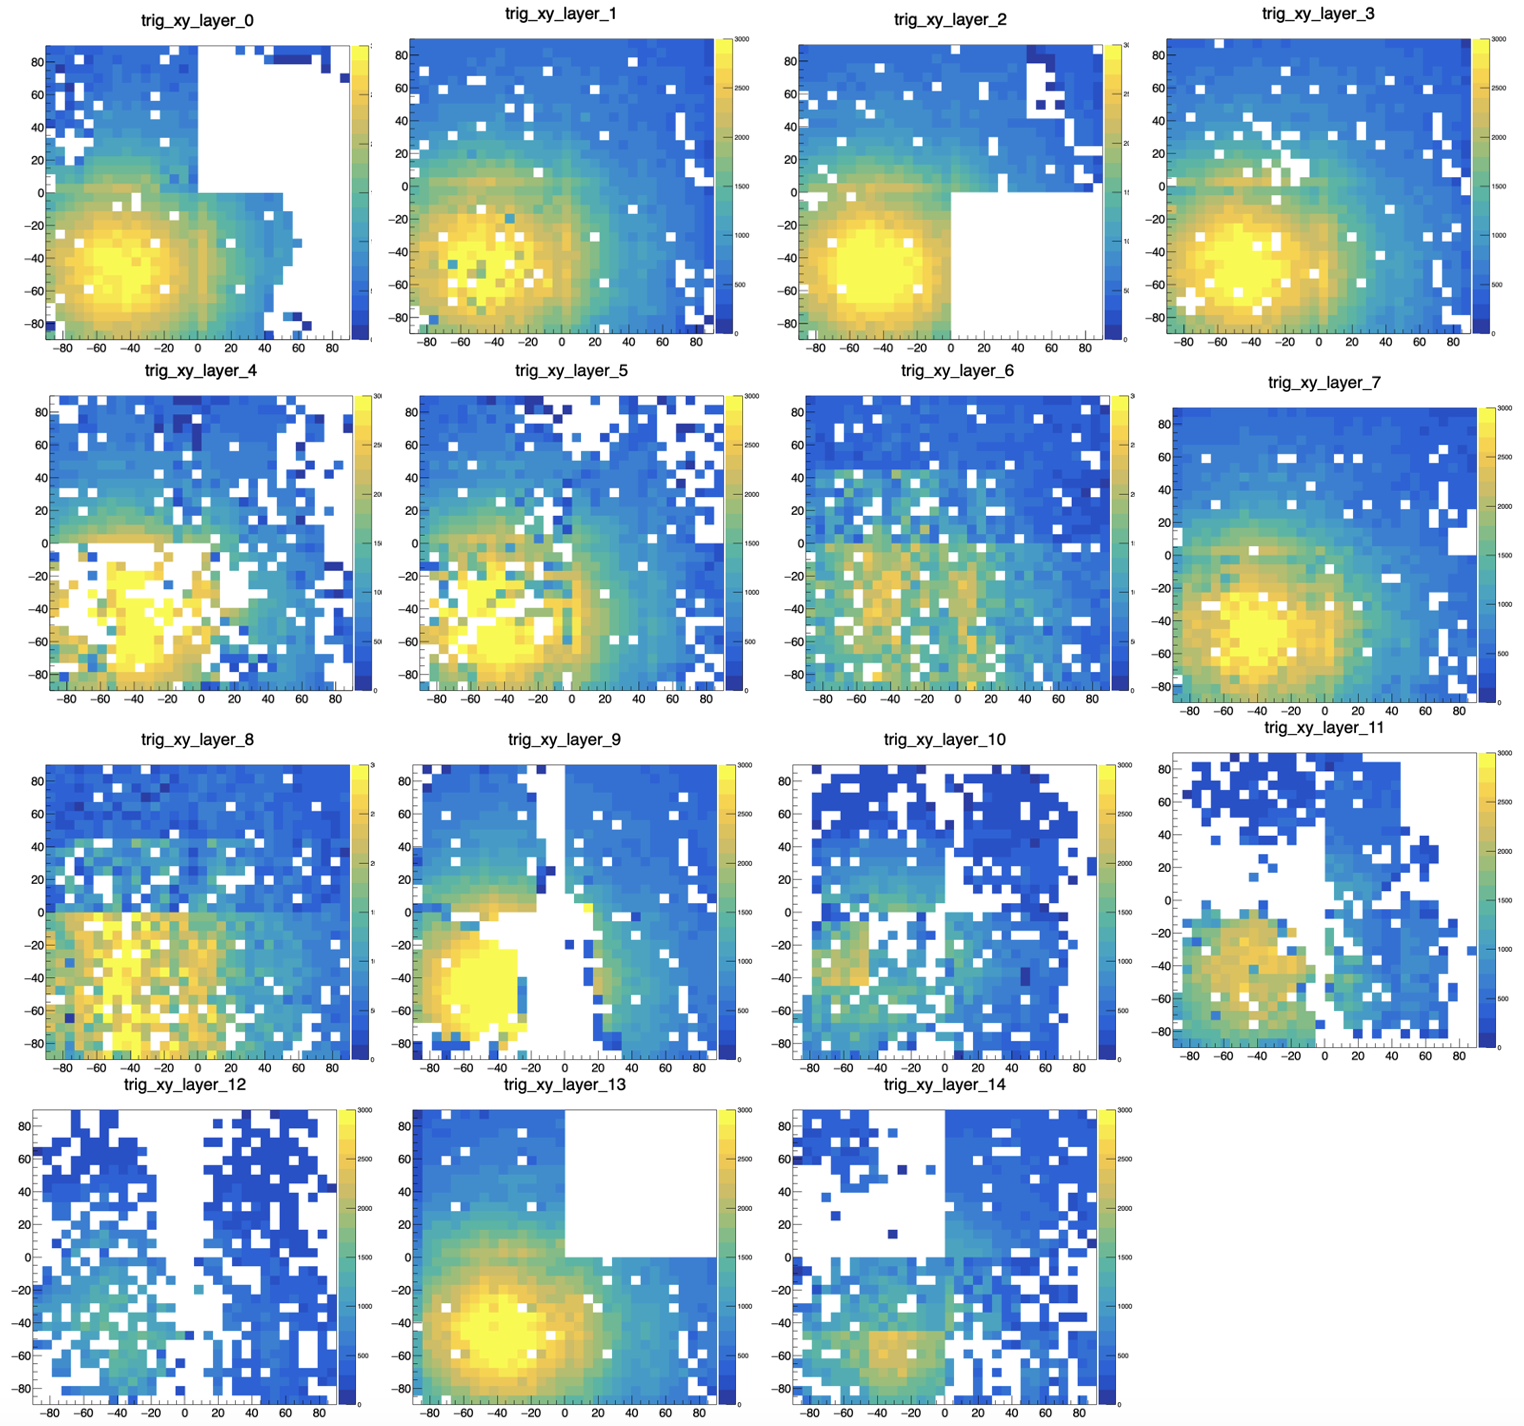
\includegraphics[keepaspectratio, scale=0.45]
 	{Figure/Beamtest/trigger.png}
 		\caption[Triggerのマップ]{各層におけるTriggerの発生数}
		\label{trigger}
\end{center}
\end{figure}
\begin{figure}[H]
\begin{center}
 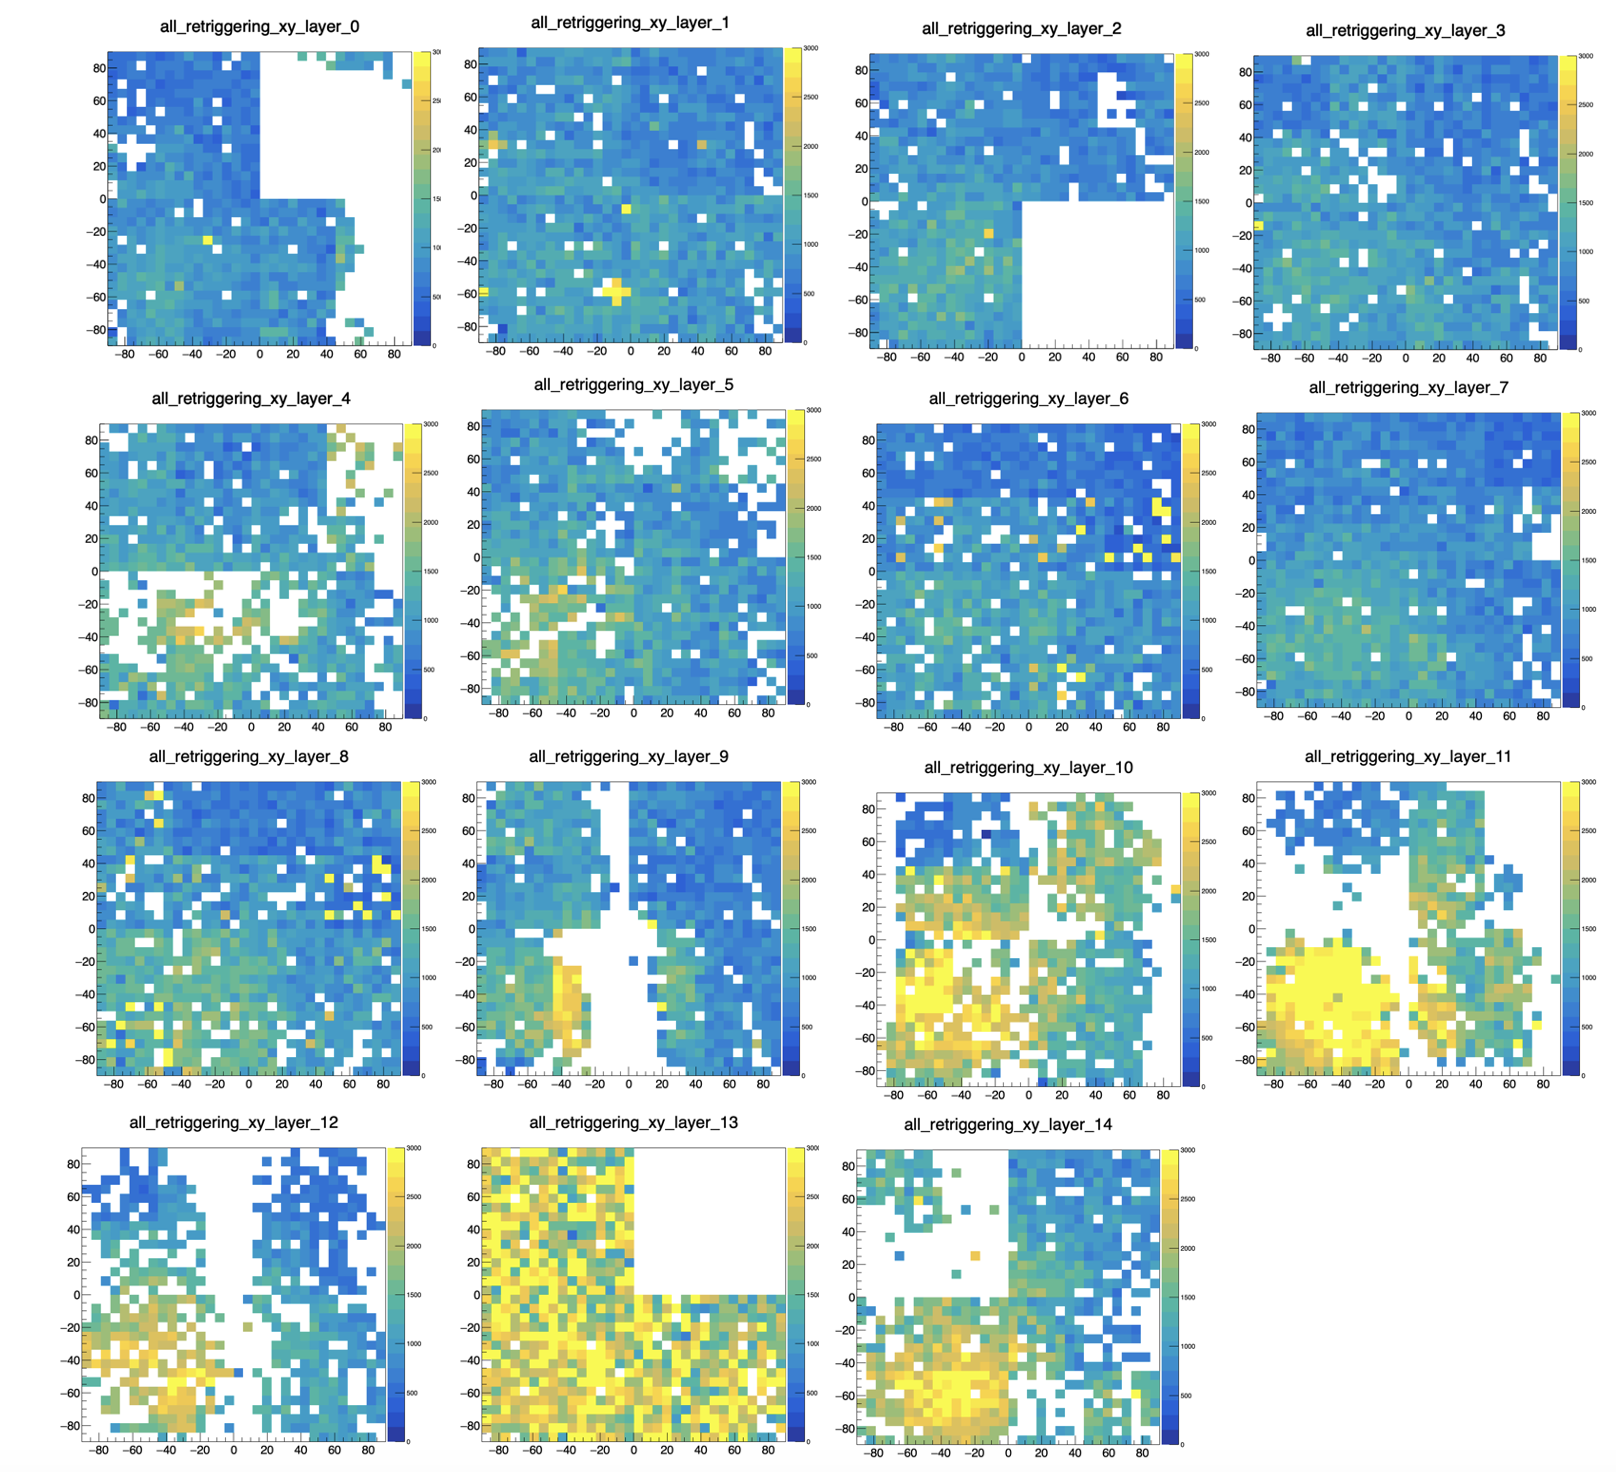
\includegraphics[keepaspectratio, scale=0.45]
 	{Figure/Beamtest/retrigger.png}
 		\caption[Retriggeirngのマップ]{各層におけるRetriggeringの発生数}
		\label{retrigger}
\end{center}
\end{figure}

上記の結果より、RetriggeringはTrigger数の多い箇所で発生数が多く、またそこでは同時にダブルぺデスタルが発生している可能性が高いことを推測することができる。また、配線を改善したFEVのアップデートでは、ダブルぺデスタルだけでなくRetriggeringの発生数も抑えることができていることが確認できた。